% chap4.tex (Definitions and Theorem)

\chapter{Storage Optimization for Trace Data} \label{MostNarrowEasy}

In this chapter, we explore optimization of provenance graph size using pruning approach. 

%\section{A Policy-Based Approach for Provenance Storage}

\section{Introduction}

%Data provenance captures information flow of across a systems which has applications in forensic analysis, intrusion detection and to scientific research for experiment reproducability. Due to the benefit provenance offers, it has received significant amounts of attention from the scientific community which has led to the development of various provenance-aware applications. For example, PASS \cite{muniswamy_reddy} and HiFi \cite{hi_fi}, both linux based provenance collection system which captures interaction between file level interactions and system calls. Chimera \cite{chimera} and myGrid,  a provenance collection system for scientific workflow reproducibility. These and many more are some of the applications that have been developed as a result of provenance proliferation. In certain cases, provenance generated might be uninteresting to the application. However, one of the major challenge faced by provenance-aware systems is that provenance data incurs additional storage overhead. That is, provenance can easily generate more data than the data in which provenance is is being captured. Our framework, PAIoT is no exception.   The resource constraints imposed on the sensor-actuator and the device layer of the IoT architecture makes storing this data a more challenging task. Table 1 outlines trace and provenance data generated at various event size. We can observe a linear progression in trace and provenance size.  Additionally, due to the large influx of real-time data generated from sensors and actuators, and preliminary results derived, we envision large amounts of provenance data generated from our provenance collection framework.  

%Motivated by the need to provide an optimized storage for provenance data generated, we address the issue of device storage optimization at the trace level by pruning events based on predefined heuristics. Pruning involves the elimination of irrelevant trace data thereby giving way to incoming data. The resultant is a more efficient and sparse representation of the original input trace
%
%The definition of what trace to prune is a challenging task and is often application dependent.



%In this chapter, we make the following contributions:
%
%\begin{itemize}
%
%\item To address the storage issue with automatic provenance collection, we integrate the use data pruning at the trace level to reduce the size of trace data generated. 
%
%\item We develop a data pruning algorithm which produces human readable and semantically meaningful summarized provenance graphs.
%
%
%\end{itemize}

A major challenge faced by any provenance capture system is that provenance data incurs additional storage overhead \cite{issue_provenance}. That is, provenance can easily generate more data itself than data about which provenance is being captured. This storage problem could lead to rapid decline in system performance both in collection and analysis of provenance. Prov-CPS is no exception. Furthermore, the resource constraints imposed on CPS devices further exacerbates the challenge. Table \ref{table:prov_growth} outlines trace and provenance data generated for increasing counts of trace events of a sample application that generates temperature data. 

%We can observe a linear progression in trace and provenance size with respect to time.

%\begin{table}[!b]
%\caption{Trace data size as number of trace increases }
%\label{table:prov_growth}
%\begin{center}
% \begin{tabular}{||c| c| c| c||} 
% \hline
% \textbf{Trace Events} & \textbf{Trace Size (KiB)} & \textbf{Provenance Size (KiB)}  \\ [0.5ex] 
% \hline\hline
% 200 & 8.2 & 25.6 \\ 
% \hline
% 500 & 25.6 & 318.4 \\
% \hline
% 1000 & 51.2 & 642.8 \\
% \hline
% 1500 & 76.8 & 966.5 \\
% \hline
%\end{tabular}
%
%\end{center}
%\end{table}


\begin{table}[!b]
\caption{Trace data size as number of trace increases }
\label{table:prov_growth}
\begin{center}
 \begin{tabular}{||c| c| c| c||} 
 \hline
 \textbf{Trace Events} & \textbf{Trace Size (KiB)} \\ [0.5ex] 
 \hline\hline
 200 & 8.2 \\ 
 \hline
 500 & 25.6 \\
 \hline
 1000 & 51.2 \\
 \hline
 1500 & 76.8 \\
 \hline
\end{tabular}

\end{center}
\end{table}



\subsection{Trace event cost estimation}
To verify the hypothesis that there exists a linear growth in trace and provenance data generated, we provide formulas to estimate the size of provenance and trace events data generated by a device. To calculate the total storage size of trace data generated on a device, we estimate the size of an event. Every event consists of a finite set of event fields such a controller, producer, action. 

%However, information contained in these fields might be encoded as string identifiers with varied sizes. These values can be encoded into a fixed amount of characters and integers. 

The total size of a trace data can be calculated using the function:  \[T_{size} = N_{events} \times K\] where $T_{size}, N_{events}$, represents trace size, and number of events respectively.  $K$ represents the sum of the size of all of the fields contained in an event trace:  \[ K = t_{size} + d_{size}+ a_{size} + c_{size} + p_{size}\] Additionally, given the size of a device, $D_{size}$, the number of trace events that can be stored on a device, $D_{capacity}$, is derived using the function:
%given the number of trace contained in a file
\[ D_{capacity} = \frac{D_{size}}{K} \]


%The total graph size can be calculated by using the formula: \[ G_{size} = \sum{(N_{events} \times (S_{entity} + S_{action}+ X)) + S_{producer} + S_{consumer} } \] where $S_{entity}, S_{producer}$ represents the size of an entity and activity node and $X$ represents the sum of the size of a fixed set of edges per trace event. 


Figure \ref{fig:prov_trace} illustrates the graph of the estimated and actual trace generated from the initial analysis in Table \ref{table:prov_growth}. For calculating the cost of trace events data, the size of each component contained in the trace event is set to 10 bytes. We can observe a linear growth between the estimated and generated data for trace events. 


%\begin{figure*}[!htb]
% 
%\centering
%\subfloat[trace size per events]{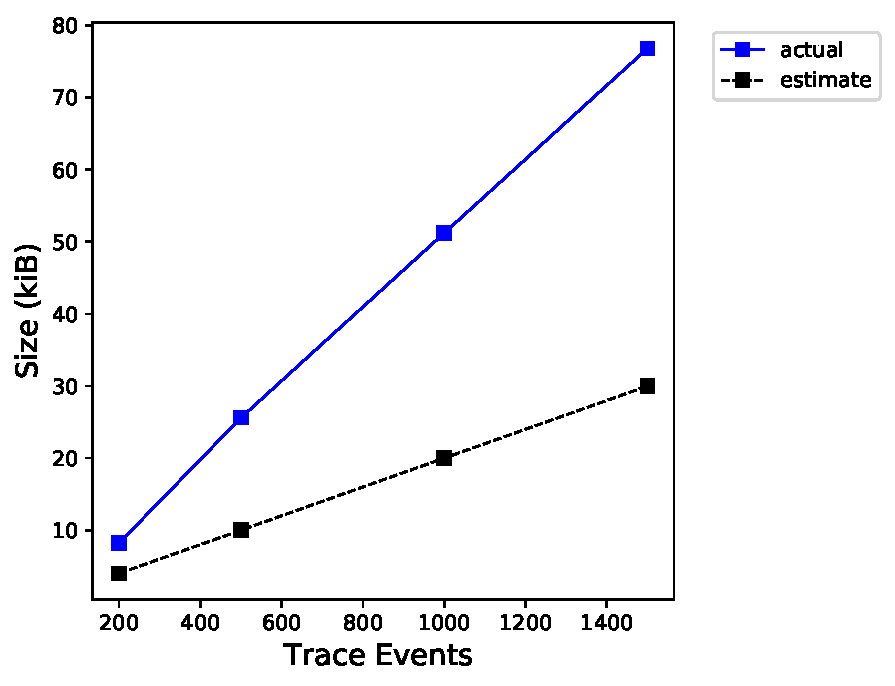
\includegraphics[width=.45\textwidth]{output_trace.pdf}\label{fig:storage_trace}}
%\qquad
%\subfloat[provenance graph size per events]{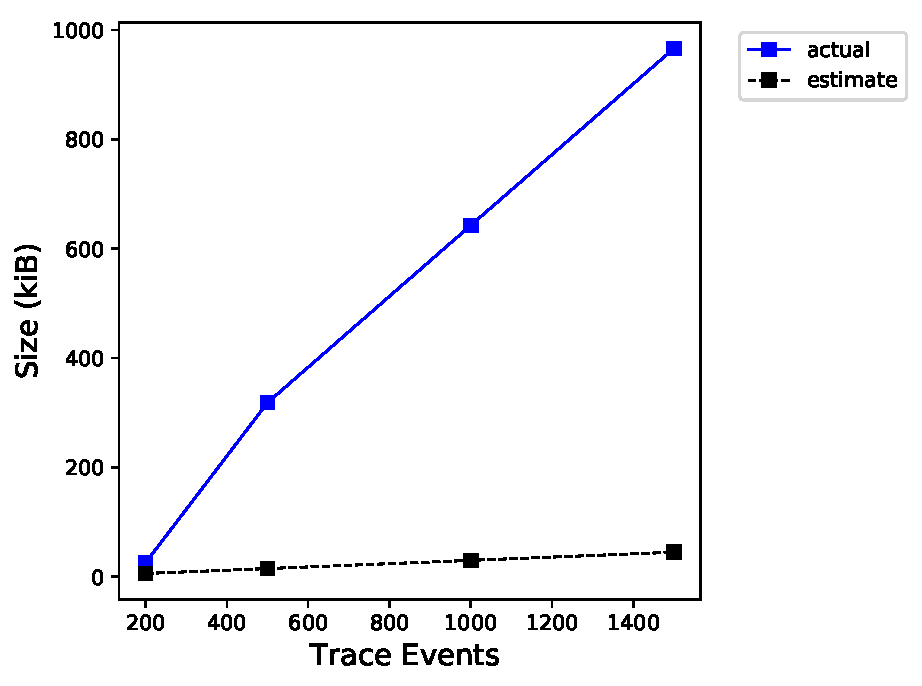
\includegraphics[width=.45\textwidth]{output_prov_1.pdf}\label{fig:storage_prov}}
%%\hfill
%%\subfloat[ROC with Priority Pruning]{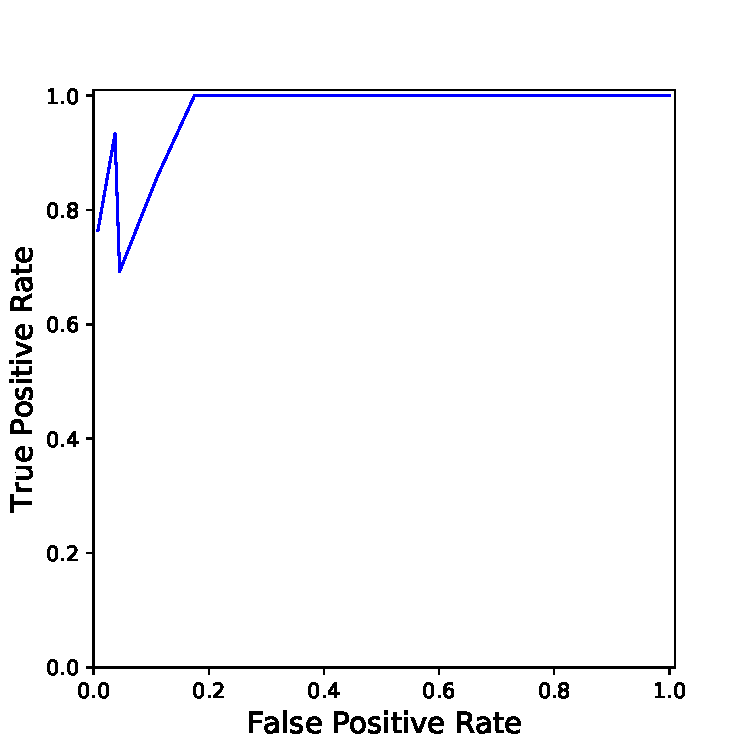
\includegraphics[width=.3\textwidth]{roc_curve_2.pdf}\label{fig:storage_growth}}
%\caption{Storage growth per trace events.}
%\label{fig:prov_trace}
%
%\end{figure*}


\begin{figure}[tbh!]
\begin{center}
%\includegraphics[width=\textwidth]{vector3.pdf}
%\includegraphics[width=\textwidth]{vector5.pdf}
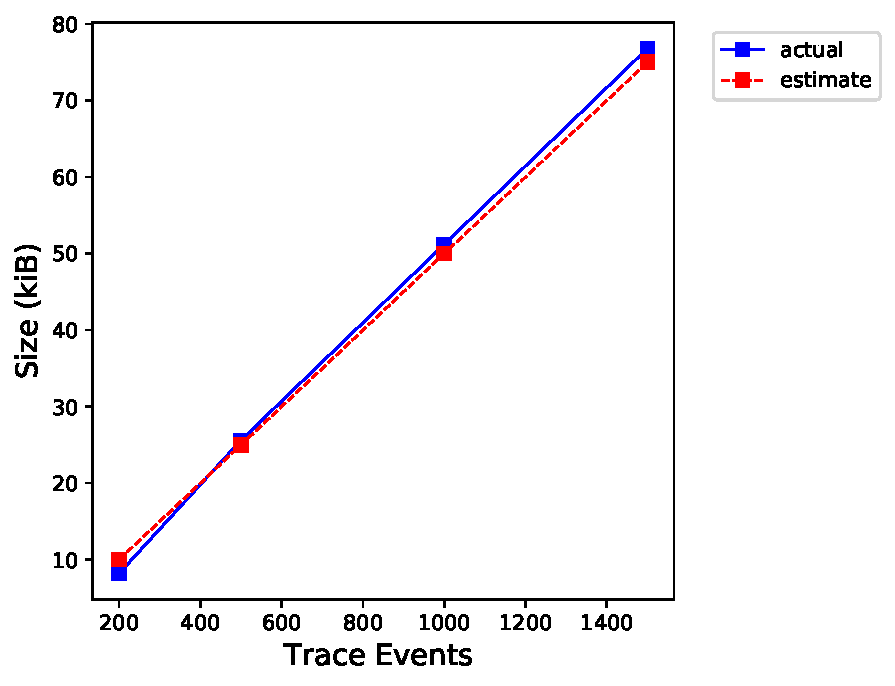
\includegraphics[width=.6\textwidth]{output_prov_trace.pdf}
\end{center}
\caption{Storage growth per trace events. }
\label{fig:prov_trace}
\end{figure}



%It is important to note that the estimated provenance graph is an approximate scalar multiple of the actual graph size which is due to the additional storage overhead from provenance graphs serialization to JSON. 

%The Algorithm defines a fixed set of edges per trace events and each event creates a new node. 


Motivated by the need to provide an optimized storage for provenance data generated, we address the issue of device storage at the trace level by pruning events based on predefined heuristics. Pruning is defined as eliminating unwanted events in a trace to optimize storage space. %We develop a data pruning algorithm which produces human readable and semantically meaningful provenance trace. The resultant is a more efficient and sparse representation of the original input trace. More information on the pruning heuristic used is discussed in section \ref{Pruning}. 


 

\section{Types of Provenance Pruning} 
To determine what data to prune is a challenging task and often application dependent.  %For example, provenance data might be considered uninteresting until it has been modified by a malicious instance. 
%braun2006issues
Based on the current state of the art, the common approaches to data pruning are:
 
\textbf{Pruning at collection} removes provenance during or before the collector stores it. For example, an application might decide to eliminate repeated trace data as they are generated, or a system-call provenance collector in an operating system kernel might ignore user configuration and temporary files that are unnecessary for the provenance application use case.

\textbf{Pruning after collection}  involves removing unwanted provenance information after provenance has been saved to a storage system. %For example, we can target attributes that are found in every trace event.

\textbf{Policy-based pruning} \cite{Bates:2015:TOY:2814579.2814586} involves the use of user-specified conditions (expressed as a policy) to determine data to prune. Policy offers a flexible method of pruning, but requires a robust policy language to express policy decisions, which often could be a challenge to design. A policy is evaluated by a decision point  that returns accept or deny. %So far, to the best of our knowledge,~\cite{bates_towards_2013} is the only policy-based approach described in the literature.

%\textbf{Graph Summarization} \cite{compressing_graph, Tian, Navlakha} involves aggregating graph nodes and edge relationships based on similar attributes without loosing information contained in the original graph. This reduces the size of the original graph while preserving the structural pattern of node and edge relationships.  

\textbf{Compression}~\cite{xie11-tapp,hussain_secure_2014, 7038199} involves reducing the size required to represent a data value. Provenance compression may be applied to the provenance or to its graph structure. The use of lossy or lossless techniques can be employed in provenance pruning, but the existing literature advocates for lossless approaches.

\textbf{Graph summarization} involves aggregating graph nodes and edge relationships based on similar attributes without loosing information contained in the original graph. This reduces the size of the original graph while preserving the structural pattern of node and edge relationships. The structural pattern of provenance graph consists of homogeneous nodes (i.e., entity, agent, activity) which can be harnessed to provide attribute-based summarization to an original graph structure. Summarization improves graph visualization and allows for better understanding of graph structures and relationship between various node and edge interactions.

\section{Pruning in Prov-CPS} \label{Pruning}
Our approach involves pruning at collection by selectively dropping events from the set of captured traces. We introduce two techniques for provenance pruning: first-in, first-out (FIFO) and prioritized.  
\begin{enumerate}

%\item\textbf{Least-$k$ queue-based pruning:}  

\item\textbf{FIFO pruning:}  
  FIFO is the na\"ive approach that uses the natural order of arrival time to select events to discard. As trace events are generated they are added to a FIFO. Once the queue has reached its capacity, each new trace event causes the oldest trace event in the FIFO to be eliminated. An advantage of FIFO pruning is that it can be implemented without application knowledge. A disadvantage is that it is not selective in what it discards, and if provenance becomes more important (for a given provenance application) as it becomes older, then FIFO is not a good choice.
%  Each event traced is stored in a queue, $Q$ where $Q= \{ q_1,...,q_n\}$. We define the queue capacity, $c$ as the maximum size of the queue. When the size of $Q$ exceeds $c$, the last $k$ element is truncated from $Q$ and the incoming trace data is appended to the end of $Q$. $k$ can be defined by application logic or by the user.

\item \textbf{Prioritized pruning:}
The prioritized approach assigns a priority value to each event as it is traced based on an application defined priority, thus it extends the definition of the trace event with an additional field for the priority value. Although application knowledge is required to determine the priority of each event, many CPS application domains include natural priority values that can be immediately leveraged by the provenance application. With this approach, lower priority events are discarded from the set of trace events first. A drawback of this approach is the cost needed to sort trace events when there are many priority values.

% This technique is similar to the na\"ive approach however, the key difference is the use of application defined logic contained in each trace event as a means to assign priority value.
% For example, in a CAN protocol bus~\cite{can_bus}--a popular messaging protocol used by in-vehicular devices (Electronic Control Units) to communicate with each other, two messages transmitted on a can bus at the same time undergo an arbitration process which involves choosing what messages are first transmitted on the network bus. Priority is given to an ECU with low id. That is, an id with a lower number always wins the arbitration process. This idea can be leveraged to perform pruning where messages with higher message ids are placed at the end of the queue. Once the queue reaches its capacity, $k$ messages are truncated to give room for new messages which are appended at the end of the queue.
\end{enumerate}

\subsection{Complexity analysis}
\textbf{FIFO Pruning} is implemented using a queue data structure. This takes constant time $O(1)$ to insert and delete events from queue. Since there are $n$ elements contained in the queue, the worst case space utilized is $O(n)$. \textbf{Priority-based pruning} is implemented using a heap data structure. It takes $O(\log{}n)$ to insert and delete elements contained in the heap with a space complexity of $O(n)$.

\section{Summary}
This chapter motivates the need for storage optimization in PROV-CPS. Two pruning heuristics, FIFO and Priority-based pruning, were proposed to address the issue of the storage overhead generated by PROV-CPS. The next chapter introduces a provenance-based anomaly detection system for the detection of anomalous instances through information flow of device events. 

%Graph summarization is a process of aggregating graph nodes and edge relationships based on similar attributes without loosing information contained in the original graph. This reduces the size of the original graph while preserving the structural pattern of node and edge relationships. The structural pattern of provenance graph consists of homogeneous nodes (i.e., entity, agent, activity) which can be harnessed to provide attribute-based summarization to an original graph structure. Summarization improves graph visualization is allows for better understanding of graph structures and relationship between various node and edge interactions. One major challenge with summarization is dealing with the complexity and volume of data generated and also with complex dependency relationships that exists between nodes.
%
%
%Graph summarization also has applications in clustering, classification, outlier detection \cite{Smets2011TheOO}, graph query optimization and understanding the interaction of large graph dataset through visualization.
%
%For this dissertation, we are focused on using graph summarization of provenance graphs for storage optimization.
%
%
%% Summarization allows users to make sense of data through visualization and also as a storage optimization technique.
%
%
%
%In this chapter, we make the following contributions:
%
%\begin{itemize}
%
%\item To address the storage issue with automatic provenance collection, we integrate the use of graph summarization by grouping specific node/edge relationship to reduce the original graph size. 
%
%\item We develop a graph summarization method which produces human readable and semantically meaningful summarized provenance graphs.
%
%\item We evaluate our provenance summarization algorithm on a dataset from an automotive domain. Our experiment calculates the percentage of storage savings(i.e., size difference) by comparing the size of the resulting summarized provenance graph to the original graph.
%\end{itemize}
%
% The remaining part of this chapter are outlined as follows. Section 2 discusses types of graph summarization, section 3 talks about our rational for graph summarization. 
%
%  
% 
% \subsection{Graph Summarization Characteristics}
%
%Due to the intricate dependency relationship that might exist between node contained in a provenance graphs and also based on the application use case, most provenance graphs are input to some real time computation on the provenance graphs, a provenance graph summary should satisfy the following characteristics:
%
%\begin{itemize}
%\item \textbf{Completeness.} A summarized graph should reproduce provenance data as contained in the original graph in a manner that preserves information contained in the node and edges of the original graph without loosing information contained. 
%
%\item \textbf{Efficiency.} Since provenance data typically consists of massive dataset of graph data, a provenance summary should produce a concise representation of the original graph which helps speed up graph processing.  
%
%\item \textbf{Queryable.}  A summarized provenance graph should represent a compact representation of the original graph which can be efficiently queried without loss of information.  
%
%\end{itemize}
%
%We satisfy the requirements listed above by aggregating the contents of similar nodes contained in the provenance graph based on defined attributes. More information on our approach is discussed in section \ref{}
%
%
%
%\subsection{Graph Summarization Techniques}
% 
%% Types of graph summarization are outlined below as follows: 
%
%There has been a considerable amount of prior work done on graph summarization \cite{grass, compressing_graph, Tian, Navlakha, hussain_secure_2014} most of which are application specific. Some of the prior work focuses on storage space reduction \cite{grass, Tian, Navlakha} using attributes while others focuses on bit compression \cite{compressing_graph, hussain_secure_2014} and  techniques. Below are the types of summarization technique used based on prior work.
%
%\begin{itemize}
%
%\item \textbf{Grouping or aggregation based approach.} This is one of the most popular approach in which nodes and edges with similar attributes are aggregated. Grouping based approach is classified into two categories:
%
%\begin{itemize}
%
%\item \textit{Node grouping} involves two types: Clustering approach in which node in densly located node clusters are grouped into a single node referred to as a super-node. The other approach involves grouping nodes with similar attributes into a super-node based on a defined attribute or structure. 
%
%\item \textit{Edge grouping} involves aggregating edges with similar attributes into compressor or virtual nodes. Compression in this case refers to replacing a set of edges into a node. 
%
%\end{itemize}
%
%\item \textbf{Compression-based approach} employs the use of compression algorithms (lossy and lossless approach) to reduce the number of bits required for each node and edge contained in the provenance graph.
%
%\item \textbf{Simplication or prunning approach} eliminates unimportant nodes or edge relationship contained in a graph. The challenge is in determining what is considered unimportant which is often times application specific. The resultant summarized graph produced is a sparse representation of the original graph.
%
%\item \textbf{Statistical-based approach.} employs the use of statistical methods such degree distribution, hop-plot, and clustering co-efficient for edges and node aggregation.
%
%\end{itemize}
%
%\section{Comparing graph summarization to other storage optimization approach}
%
%\begin{itemize}
%
%\item \textbf{\textit{Policy-based prunning}}: There has been a limited amount of prior work on policy-based pruning for provenance. Bates et al \cite{Bates:2015:TOY:2814579.2814586}. proposed a policy based approach which enforces ppruning at the OS based on MAC policies. Summarization helps reduce storage cost while discovering structural patterns that exists in the original input graph. With policy-based pruning, lossy optimization techniques is often utilized as a means of elimimating unimportant information contained in the provenance graph. The definition of data considered unimportant is relative and domain specific. One might argue that pruning provenance data removes provenance data originality. (i.e., the lineage of data has been tampered with) since it deletes from the history. 
%
%
%\item \textbf{\textit{Compression}}: Although summarization and compression might seem related since they both involve combining nodes and edges with a resulting space optimized graph, they are quite different. Compression focuses on minimizing graph edges without the need to produce a summarized graph. For example, a compression techniques can be applied to a whole graph without preserving graph structure. Graph summarization on the other hand leverages compression to generate an efficient graph summary from an input graph while maintaining structural patterns that might exist in the original graph.
%
%\end{itemize}
%
%
%\par Both policy-based prunning and compression are complementary to graph summarization. That is, both are more effective when used in combination with graph summarization techniques. To this effect, our approach utilizes a combination of node aggregation, bit compression and pruning techniques to ensure optimal space savings.
%
%
%\section{Our Approach}
%
%Provenance graph contains redundant information such as edge and node labels. Also, we group nodes based on activity type with time dependency. That is nodes that occur successively with the same activity are grouped as one super-node. Also, we introduce the use of the pruning approach whereby we remove nodes based on user specified attributes.Our algorithm makes use of bit compression, graph aggregation and prunning approach to optimize space savings.
%
%
%
%
%
%\section{Related Work}
%
%
%\section{Experimental Evaluation}

%
%Since organizations have varied provenance requirement(s), making a static provenance policy is not suitable for the IoT. Using policy for storage optimization is slightly different from the typical use of policy in enforcing access control.  For the IoT framework, the product manufacturer is considered a policy creator. This reduces the complexity of creating and managing policy documents by the IoT device consumers. A policy creator is a user which has the right to add, delete or modify a policy document. A policy document is required to specify which provenance data to collect thereby providing storage access to provenance unlike system access control which evaluates user access rights to view a resource. 
%
%
%
%
%
%\par 
%
%The policy framework consists of a policy engine. The policy engine contains authorization and enforcement components that provides and enforce decisions on how provenance data should be stored. A policy document is a component of the policy framework. It identifies provenance data that is considered relevant to the IoT application. Our policy architecture is modeled using the Common Open Policy Service (COPS) Standard \cite{rfc2748}. COPS consists of components for policy generation, evaluation and enforcement. The Policy Enforcement Point (PEP) enforces decisions received from the Policy Decision Point (PDP). The PDP evaluates policies and generates decision based on the evaluation. The model can be extended to include a secondary decision point (SDP) which allows for distributed policy evaluation, thus freeing up the PDP from communication bottlenecks caused by large amounts of requests received by a single PDP. Figure \ref{policy_architecture} below illustrates the system architecture of our proposed policy-based storage framework. Different layers of the IoT architecture contain different decision and enforcement components. The sensor-actuator layer of the IoT architecture is omitted because it has negligible memory resources and the  sensors and actuators are usually physically part of a device in the device layer and as such does not have any data to prune. 
%
%
%Policy document which is generated by the policy creator serves as an input to the PDP component and is evaluated at the device, gateway and cloud layer. The PEP which is involved with generating requests is located in the device and gateway layer. SDPs can be located in the gateway layer, which allows for policy evaluation without incurring additional network overhead of communicating with the PDP located in the cloud layer. 


